\documentclass[1p]{elsarticle_modified}
%\bibliographystyle{elsarticle-num}

%\usepackage[colorlinks]{hyperref}
%\usepackage{abbrmath_seonhwa} %\Abb, \Ascr, \Acal ,\Abf, \Afrak
\usepackage{amsfonts}
\usepackage{amssymb}
\usepackage{amsmath}
\usepackage{amsthm}
\usepackage{scalefnt}
\usepackage{amsbsy}
\usepackage{kotex}
\usepackage{caption}
\usepackage{subfig}
\usepackage{color}
\usepackage{graphicx}
\usepackage{xcolor} %% white, black, red, green, blue, cyan, magenta, yellow
\usepackage{float}
\usepackage{setspace}
\usepackage{hyperref}

\usepackage{tikz}
\usetikzlibrary{arrows}

\usepackage{multirow}
\usepackage{array} % fixed length table
\usepackage{hhline}

%%%%%%%%%%%%%%%%%%%%%
\makeatletter
\renewcommand*\env@matrix[1][\arraystretch]{%
	\edef\arraystretch{#1}%
	\hskip -\arraycolsep
	\let\@ifnextchar\new@ifnextchar
	\array{*\c@MaxMatrixCols c}}
\makeatother %https://tex.stackexchange.com/questions/14071/how-can-i-increase-the-line-spacing-in-a-matrix
%%%%%%%%%%%%%%%

\usepackage[normalem]{ulem}

\newcommand{\msout}[1]{\ifmmode\text{\sout{\ensuremath{#1}}}\else\sout{#1}\fi}
%SOURCE: \msout is \stkout macro in https://tex.stackexchange.com/questions/20609/strikeout-in-math-mode

\newcommand{\cancel}[1]{
	\ifmmode
	{\color{red}\msout{#1}}
	\else
	{\color{red}\sout{#1}}
	\fi
}

\newcommand{\add}[1]{
	{\color{blue}\uwave{#1}}
}

\newcommand{\replace}[2]{
	\ifmmode
	{\color{red}\msout{#1}}{\color{blue}\uwave{#2}}
	\else
	{\color{red}\sout{#1}}{\color{blue}\uwave{#2}}
	\fi
}

\newcommand{\Sol}{\mathcal{S}} %segment
\newcommand{\D}{D} %diagram
\newcommand{\A}{\mathcal{A}} %arc


%%%%%%%%%%%%%%%%%%%%%%%%%%%%%5 test

\def\sl{\operatorname{\textup{SL}}(2,\Cbb)}
\def\psl{\operatorname{\textup{PSL}}(2,\Cbb)}
\def\quan{\mkern 1mu \triangleright \mkern 1mu}

\theoremstyle{definition}
\newtheorem{thm}{Theorem}[section]
\newtheorem{prop}[thm]{Proposition}
\newtheorem{lem}[thm]{Lemma}
\newtheorem{ques}[thm]{Question}
\newtheorem{cor}[thm]{Corollary}
\newtheorem{defn}[thm]{Definition}
\newtheorem{exam}[thm]{Example}
\newtheorem{rmk}[thm]{Remark}
\newtheorem{alg}[thm]{Algorithm}

\newcommand{\I}{\sqrt{-1}}
\begin{document}

%\begin{frontmatter}
%
%\title{Boundary parabolic representations of knots up to 8 crossings}
%
%%% Group authors per affiliation:
%\author{Yunhi Cho} 
%\address{Department of Mathematics, University of Seoul, Seoul, Korea}
%\ead{yhcho@uos.ac.kr}
%
%
%\author{Seonhwa Kim} %\fnref{s_kim}}
%\address{Center for Geometry and Physics, Institute for Basic Science, Pohang, 37673, Korea}
%\ead{ryeona17@ibs.re.kr}
%
%\author{Hyuk Kim}
%\address{Department of Mathematical Sciences, Seoul National University, Seoul 08826, Korea}
%\ead{hyukkim@snu.ac.kr}
%
%\author{Seokbeom Yoon}
%\address{Department of Mathematical Sciences, Seoul National University, Seoul, 08826,  Korea}
%\ead{sbyoon15@snu.ac.kr}
%
%\begin{abstract}
%We find all boundary parabolic representation of knots up to 8 crossings.
%
%\end{abstract}
%\begin{keyword}
%    \MSC[2010] 57M25 
%\end{keyword}
%
%\end{frontmatter}

%\linenumbers
%\tableofcontents
%
\newcommand\colored[1]{\textcolor{white}{\rule[-0.35ex]{0.8em}{1.4ex}}\kern-0.8em\color{red} #1}%
%\newcommand\colored[1]{\textcolor{white}{ #1}\kern-2.17ex	\textcolor{white}{ #1}\kern-1.81ex	\textcolor{white}{ #1}\kern-2.15ex\color{red}#1	}

{\Large $\underline{10_{85}~(K10a_{86})}$}

\setlength{\tabcolsep}{10pt}
\renewcommand{\arraystretch}{1.6}
\vspace{1cm}\begin{tabular}{m{100pt}>{\centering\arraybackslash}m{274pt}}
\multirow{5}{120pt}{
	\centering
	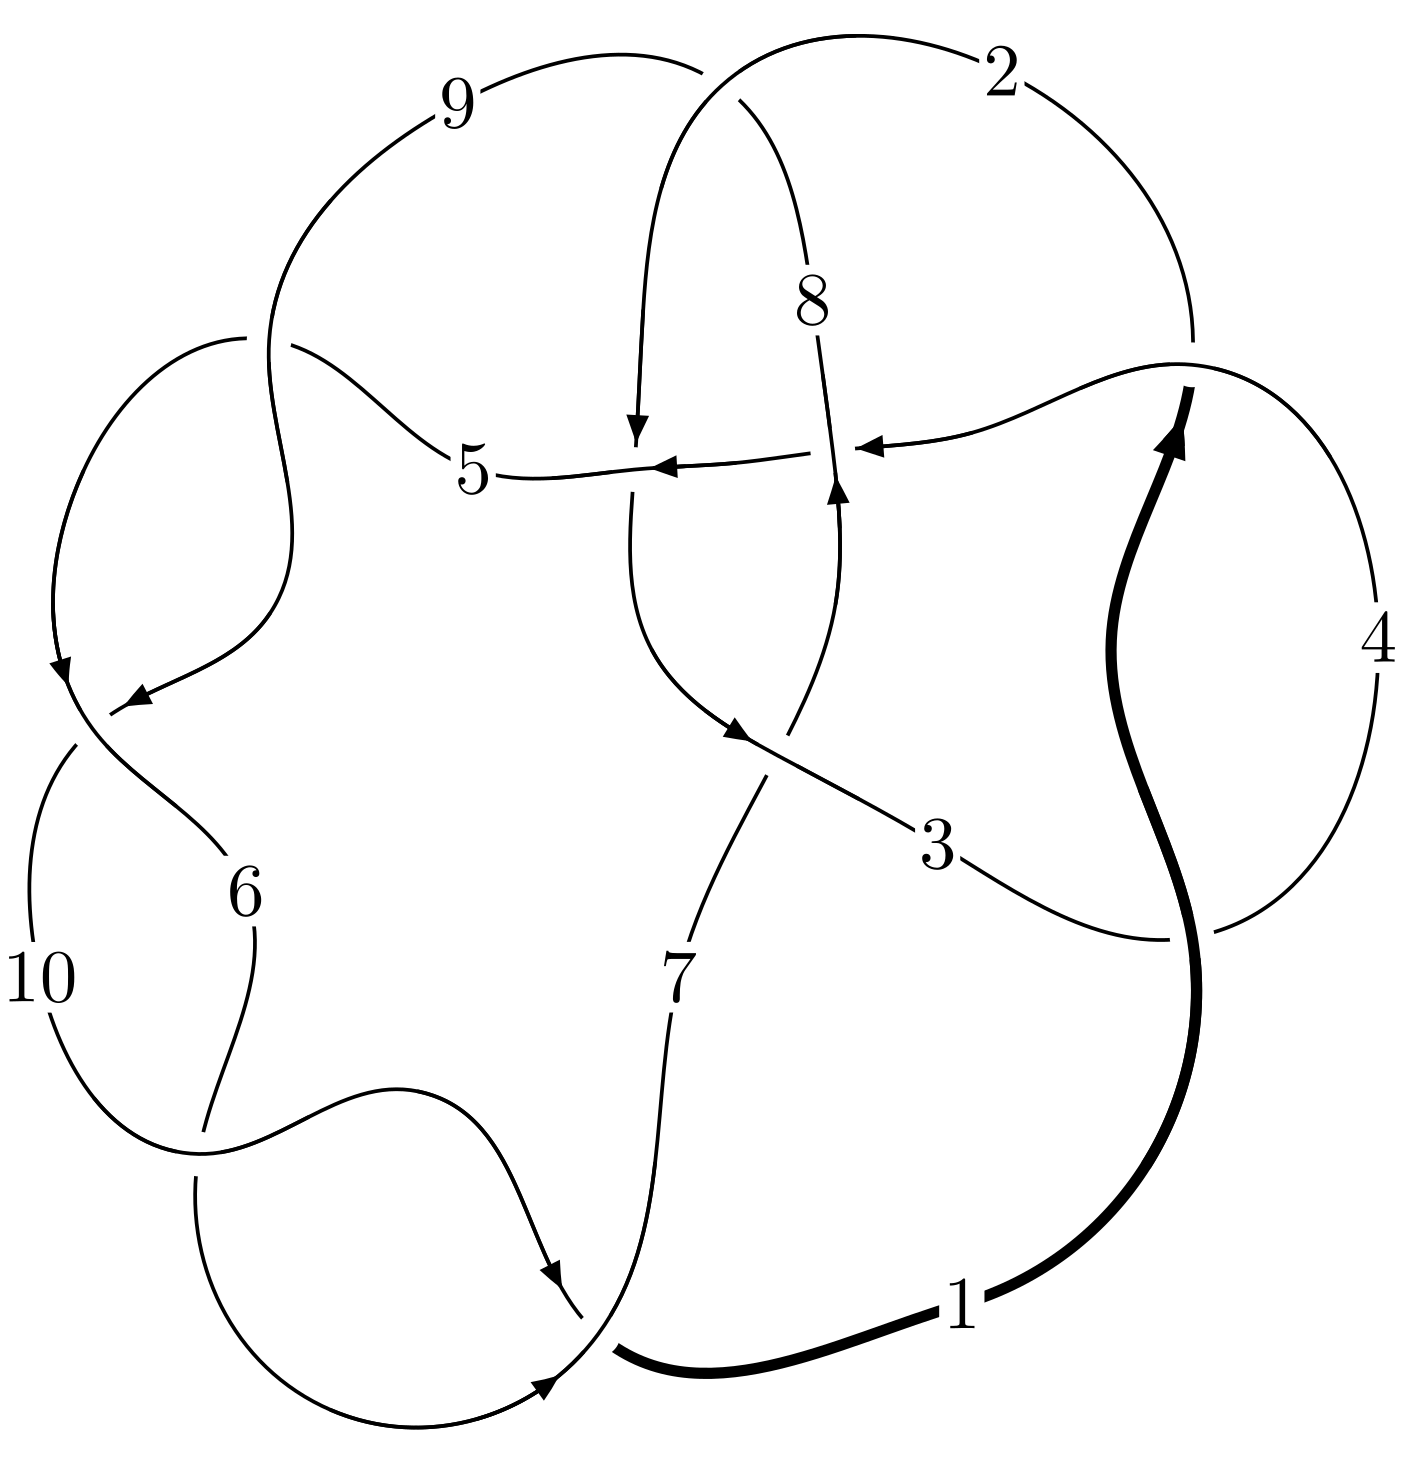
\includegraphics[width=112pt]{../../../GIT/diagram.site/Diagrams/png/169_10_85.png}\\
\ \ \ A knot diagram\footnotemark}&
\allowdisplaybreaks
\textbf{Linearized knot diagam} \\
\cline{2-2}
 &
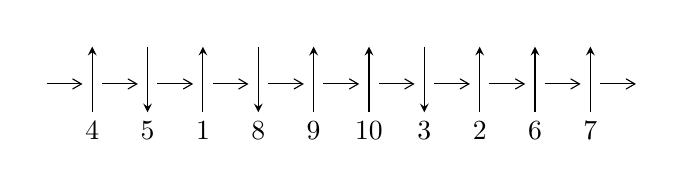
\begin{tikzpicture}[x=20pt, y=17pt]
	% nodes
	\node (C0) at (0, 0) {};
	\node (C1) at (1, 0) {};
	\node (C1U) at (1, +1) {};
	\node (C1D) at (1, -1) {4};

	\node (C2) at (2, 0) {};
	\node (C2U) at (2, +1) {};
	\node (C2D) at (2, -1) {5};

	\node (C3) at (3, 0) {};
	\node (C3U) at (3, +1) {};
	\node (C3D) at (3, -1) {1};

	\node (C4) at (4, 0) {};
	\node (C4U) at (4, +1) {};
	\node (C4D) at (4, -1) {8};

	\node (C5) at (5, 0) {};
	\node (C5U) at (5, +1) {};
	\node (C5D) at (5, -1) {9};

	\node (C6) at (6, 0) {};
	\node (C6U) at (6, +1) {};
	\node (C6D) at (6, -1) {10};

	\node (C7) at (7, 0) {};
	\node (C7U) at (7, +1) {};
	\node (C7D) at (7, -1) {3};

	\node (C8) at (8, 0) {};
	\node (C8U) at (8, +1) {};
	\node (C8D) at (8, -1) {2};

	\node (C9) at (9, 0) {};
	\node (C9U) at (9, +1) {};
	\node (C9D) at (9, -1) {6};

	\node (C10) at (10, 0) {};
	\node (C10U) at (10, +1) {};
	\node (C10D) at (10, -1) {7};
	\node (C11) at (11, 0) {};

	% arrows
	\draw[->,>={angle 60}]
	(C0) edge (C1) (C1) edge (C2) (C2) edge (C3) (C3) edge (C4) (C4) edge (C5) (C5) edge (C6) (C6) edge (C7) (C7) edge (C8) (C8) edge (C9) (C9) edge (C10) (C10) edge (C11) ;	\draw[->,>=stealth]
	(C1D) edge (C1U) (C2U) edge (C2D) (C3D) edge (C3U) (C4U) edge (C4D) (C5D) edge (C5U) (C6D) edge (C6U) (C7U) edge (C7D) (C8D) edge (C8U) (C9D) edge (C9U) (C10D) edge (C10U) ;
	\end{tikzpicture} \\
\hhline{~~} \\& 
\textbf{Solving Sequence} \\ \cline{2-2} 
 &
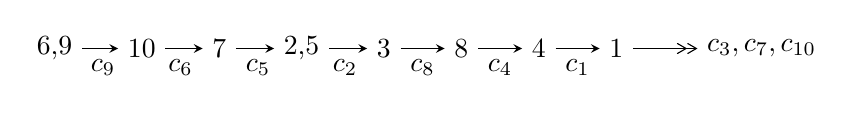
\begin{tikzpicture}[x=28pt, y=7pt]
	% node
	\node (A0) at (-1/8, 0) {6,9};
	\node (A1) at (1, 0) {10};
	\node (A2) at (2, 0) {7};
	\node (A3) at (49/16, 0) {2,5};
	\node (A4) at (33/8, 0) {3};
	\node (A5) at (41/8, 0) {8};
	\node (A6) at (49/8, 0) {4};
	\node (A7) at (57/8, 0) {1};
	\node (C1) at (1/2, -1) {$c_{9}$};
	\node (C2) at (3/2, -1) {$c_{6}$};
	\node (C3) at (5/2, -1) {$c_{5}$};
	\node (C4) at (29/8, -1) {$c_{2}$};
	\node (C5) at (37/8, -1) {$c_{8}$};
	\node (C6) at (45/8, -1) {$c_{4}$};
	\node (C7) at (53/8, -1) {$c_{1}$};
	\node (A8) at (9, 0) {$c_{3},c_{7},c_{10}$};

	% edge
	\draw[->,>=stealth]	
	(A0) edge (A1) (A1) edge (A2) (A2) edge (A3) (A3) edge (A4) (A4) edge (A5) (A5) edge (A6) (A6) edge (A7) ;
	\draw[->>,>={angle 60}]	
	(A7) edge (A8);
\end{tikzpicture} \\ 

\end{tabular} \\

\footnotetext{
The image of knot diagram is generated by the software ``\textbf{Draw programme}" developed by Andrew Bartholomew(\url{http://www.layer8.co.uk/maths/draw/index.htm\#Running-draw}), where we modified some parts for our purpose(\url{https://github.com/CATsTAILs/LinksPainter}).
}\phantom \\ \newline 
\centering \textbf{Ideals for irreducible components\footnotemark of $X_{\text{par}}$} 
 
\begin{align*}
I^u_{1}&=\langle 
60294783 u^{28}-88287773 u^{27}+\cdots+34606354 b-88284553,\\
\phantom{I^u_{1}}&\phantom{= \langle  }-32141431 u^{28}+46155247 u^{27}+\cdots+17303177 a+15723776,\;u^{29}-2 u^{28}+\cdots-5 u+1\rangle \\
I^u_{2}&=\langle 
b-1,\;a+1,\;u-1\rangle \\
\\
\end{align*}
\raggedright * 2 irreducible components of $\dim_{\mathbb{C}}=0$, with total 30 representations.\\
\footnotetext{All coefficients of polynomials are rational numbers. But the coefficients are sometimes approximated in decimal forms when there is not enough margin.}
\newpage
\renewcommand{\arraystretch}{1}
\centering \section*{I. $I^u_{1}= \langle 6.03\times10^{7} u^{28}-8.83\times10^{7} u^{27}+\cdots+3.46\times10^{7} b-8.83\times10^{7},\;-3.21\times10^{7} u^{28}+4.62\times10^{7} u^{27}+\cdots+1.73\times10^{7} a+1.57\times10^{7},\;u^{29}-2 u^{28}+\cdots-5 u+1 \rangle$}
\flushleft \textbf{(i) Arc colorings}\\
\begin{tabular}{m{7pt} m{180pt} m{7pt} m{180pt} }
\flushright $a_{6}=$&$\begin{pmatrix}0\\u\end{pmatrix}$ \\
\flushright $a_{9}=$&$\begin{pmatrix}1\\0\end{pmatrix}$ \\
\flushright $a_{10}=$&$\begin{pmatrix}1\\- u^2\end{pmatrix}$ \\
\flushright $a_{7}=$&$\begin{pmatrix}u\\- u^3+u\end{pmatrix}$ \\
\flushright $a_{2}=$&$\begin{pmatrix}1.85755 u^{28}-2.66744 u^{27}+\cdots+14.0229 u-0.908722\\-1.74230 u^{28}+2.55120 u^{27}+\cdots-12.6457 u+2.55111\end{pmatrix}$ \\
\flushright $a_{5}=$&$\begin{pmatrix}- u\\u\end{pmatrix}$ \\
\flushright $a_{3}=$&$\begin{pmatrix}1.82836 u^{28}-2.55221 u^{27}+\cdots+13.5669 u-0.794482\\-1.71312 u^{28}+2.43597 u^{27}+\cdots-12.1898 u+2.43687\end{pmatrix}$ \\
\flushright $a_{8}=$&$\begin{pmatrix}3.97113 u^{28}-4.76259 u^{27}+\cdots+10.6810 u-4.64851\\-4.16350 u^{28}+4.96257 u^{27}+\cdots-16.5831 u+4.96513\end{pmatrix}$ \\
\flushright $a_{4}=$&$\begin{pmatrix}-1.79416 u^{28}+2.57695 u^{27}+\cdots-12.7088 u+1.57715\\1.79416 u^{28}-2.57695 u^{27}+\cdots+12.7088 u-2.57715\end{pmatrix}$ \\
\flushright $a_{1}=$&$\begin{pmatrix}- u^2+1\\u^4-2 u^2\end{pmatrix}$\\&\end{tabular}
\flushleft \textbf{(ii) Obstruction class $= -1$}\\~\\
\flushleft \textbf{(iii) Cusp Shapes $= \frac{289657216}{17303177} u^{28}-\frac{414590110}{17303177} u^{27}+\cdots+\frac{1326964710}{17303177} u-\frac{307662332}{17303177}$}\\~\\
\newpage\renewcommand{\arraystretch}{1}
\flushleft \textbf{(iv) u-Polynomials at the component}\newline \\
\begin{tabular}{m{50pt}|m{274pt}}
Crossings & \hspace{64pt}u-Polynomials at each crossing \\
\hline $$\begin{aligned}c_{1},c_{3}\end{aligned}$$&$\begin{aligned}
&u^{29}+2 u^{28}+\cdots-9 u+1
\end{aligned}$\\
\hline $$\begin{aligned}c_{2}\end{aligned}$$&$\begin{aligned}
&u^{29}-5 u^{28}+\cdots+2 u+2
\end{aligned}$\\
\hline $$\begin{aligned}c_{4}\end{aligned}$$&$\begin{aligned}
&u^{29}+2 u^{28}+\cdots+u+1
\end{aligned}$\\
\hline $$\begin{aligned}c_{5},c_{6},c_{9}\\c_{10}\end{aligned}$$&$\begin{aligned}
&u^{29}-2 u^{28}+\cdots-5 u+1
\end{aligned}$\\
\hline $$\begin{aligned}c_{7}\end{aligned}$$&$\begin{aligned}
&u^{29}-4 u^{27}+\cdots-277 u+173
\end{aligned}$\\
\hline $$\begin{aligned}c_{8}\end{aligned}$$&$\begin{aligned}
&u^{29}-2 u^{28}+\cdots-51 u+1
\end{aligned}$\\
\hline
\end{tabular}\\~\\
\newpage\renewcommand{\arraystretch}{1}
\flushleft \textbf{(v) Riley Polynomials at the component}\newline \\
\begin{tabular}{m{50pt}|m{274pt}}
Crossings & \hspace{64pt}Riley Polynomials at each crossing \\
\hline $$\begin{aligned}c_{1},c_{3}\end{aligned}$$&$\begin{aligned}
&y^{29}-24 y^{28}+\cdots+35 y-1
\end{aligned}$\\
\hline $$\begin{aligned}c_{2}\end{aligned}$$&$\begin{aligned}
&y^{29}+9 y^{28}+\cdots-8 y-4
\end{aligned}$\\
\hline $$\begin{aligned}c_{4}\end{aligned}$$&$\begin{aligned}
&y^{29}+4 y^{28}+\cdots- y-1
\end{aligned}$\\
\hline $$\begin{aligned}c_{5},c_{6},c_{9}\\c_{10}\end{aligned}$$&$\begin{aligned}
&y^{29}-36 y^{28}+\cdots- y-1
\end{aligned}$\\
\hline $$\begin{aligned}c_{7}\end{aligned}$$&$\begin{aligned}
&y^{29}-8 y^{28}+\cdots-224637 y-29929
\end{aligned}$\\
\hline $$\begin{aligned}c_{8}\end{aligned}$$&$\begin{aligned}
&y^{29}-36 y^{28}+\cdots+2499 y-1
\end{aligned}$\\
\hline
\end{tabular}\\~\\
\newpage\flushleft \textbf{(vi) Complex Volumes and Cusp Shapes}
$$\begin{array}{c|c|c}  
\text{Solutions to }I^u_{1}& \I (\text{vol} + \sqrt{-1}CS) & \text{Cusp shape}\\
 \hline 
\begin{aligned}
u &= -0.945899 + 0.527377 I \\
a &= -1.42859 - 0.46825 I \\
b &= \phantom{-}1.23966 - 0.80863 I\end{aligned}
 & \phantom{-}5.88176 - 9.11420 I & \phantom{-}9.68617 + 7.34304 I \\ \hline\begin{aligned}
u &= -0.945899 - 0.527377 I \\
a &= -1.42859 + 0.46825 I \\
b &= \phantom{-}1.23966 + 0.80863 I\end{aligned}
 & \phantom{-}5.88176 + 9.11420 I & \phantom{-}9.68617 - 7.34304 I \\ \hline\begin{aligned}
u &= \phantom{-}0.919400 + 0.642162 I \\
a &= -0.315900 + 0.817663 I \\
b &= \phantom{-}0.838796 - 0.254515 I\end{aligned}
 & \phantom{-}5.23846 + 0.21078 I & \phantom{-}14.1588 + 0.1661 I \\ \hline\begin{aligned}
u &= \phantom{-}0.919400 - 0.642162 I \\
a &= -0.315900 - 0.817663 I \\
b &= \phantom{-}0.838796 + 0.254515 I\end{aligned}
 & \phantom{-}5.23846 - 0.21078 I & \phantom{-}14.1588 - 0.1661 I \\ \hline\begin{aligned}
u &= -0.852692 + 0.102964 I \\
a &= -2.16375 + 1.13712 I \\
b &= \phantom{-}0.698160 - 0.148828 I\end{aligned}
 & \phantom{-}4.90102 - 1.77997 I & \phantom{-}15.0441 + 4.1634 I \\ \hline\begin{aligned}
u &= -0.852692 - 0.102964 I \\
a &= -2.16375 - 1.13712 I \\
b &= \phantom{-}0.698160 + 0.148828 I\end{aligned}
 & \phantom{-}4.90102 + 1.77997 I & \phantom{-}15.0441 - 4.1634 I \\ \hline\begin{aligned}
u &= -0.778126 + 0.317868 I \\
a &= \phantom{-}1.21478 + 0.99243 I \\
b &= -0.813260 + 0.652109 I\end{aligned}
 & \phantom{-}1.06268 - 4.13663 I & \phantom{-}7.22942 + 7.89079 I \\ \hline\begin{aligned}
u &= -0.778126 - 0.317868 I \\
a &= \phantom{-}1.21478 - 0.99243 I \\
b &= -0.813260 - 0.652109 I\end{aligned}
 & \phantom{-}1.06268 + 4.13663 I & \phantom{-}7.22942 - 7.89079 I \\ \hline\begin{aligned}
u &= \phantom{-}0.072018 + 0.813066 I \\
a &= -0.055406 - 0.155414 I \\
b &= -0.965881 - 0.630905 I\end{aligned}
 & \phantom{-}2.76973 + 4.67347 I & \phantom{-}7.79912 - 5.64410 I \\ \hline\begin{aligned}
u &= \phantom{-}0.072018 - 0.813066 I \\
a &= -0.055406 + 0.155414 I \\
b &= -0.965881 + 0.630905 I\end{aligned}
 & \phantom{-}2.76973 - 4.67347 I & \phantom{-}7.79912 + 5.64410 I\\
 \hline 
 \end{array}$$\newpage$$\begin{array}{c|c|c}  
\text{Solutions to }I^u_{1}& \I (\text{vol} + \sqrt{-1}CS) & \text{Cusp shape}\\
 \hline 
\begin{aligned}
u &= \phantom{-}1.22499\phantom{ +0.000000I} \\
a &= -0.486025\phantom{ +0.000000I} \\
b &= -0.0200655\phantom{ +0.000000I}\end{aligned}
 & \phantom{-}2.40006\phantom{ +0.000000I} & \phantom{-}1.29980\phantom{ +0.000000I} \\ \hline\begin{aligned}
u &= \phantom{-}0.696417\phantom{ +0.000000I} \\
a &= -3.92323\phantom{ +0.000000I} \\
b &= \phantom{-}3.47362\phantom{ +0.000000I}\end{aligned}
 & \phantom{-}2.85586\phantom{ +0.000000I} & -37.1850\phantom{ +0.000000I} \\ \hline\begin{aligned}
u &= \phantom{-}0.652302 + 0.186228 I \\
a &= \phantom{-}0.677568 - 0.199223 I \\
b &= -0.726039 - 0.441283 I\end{aligned}
 & \phantom{-}1.260030 + 0.425153 I & \phantom{-}8.09157 - 0.86414 I \\ \hline\begin{aligned}
u &= \phantom{-}0.652302 - 0.186228 I \\
a &= \phantom{-}0.677568 + 0.199223 I \\
b &= -0.726039 + 0.441283 I\end{aligned}
 & \phantom{-}1.260030 - 0.425153 I & \phantom{-}8.09157 + 0.86414 I \\ \hline\begin{aligned}
u &= -0.066518 + 0.465152 I \\
a &= \phantom{-}0.922681 + 0.795965 I \\
b &= \phantom{-}0.575911 + 0.420194 I\end{aligned}
 & -1.04879 + 1.39671 I & -0.58532 - 2.57538 I \\ \hline\begin{aligned}
u &= -0.066518 - 0.465152 I \\
a &= \phantom{-}0.922681 - 0.795965 I \\
b &= \phantom{-}0.575911 - 0.420194 I\end{aligned}
 & -1.04879 - 1.39671 I & -0.58532 + 2.57538 I \\ \hline\begin{aligned}
u &= -1.62115 + 0.04828 I \\
a &= -1.28657 + 0.61647 I \\
b &= \phantom{-}1.12014 - 1.06805 I\end{aligned}
 & \phantom{-}9.19873 - 1.27855 I & \phantom{-0.000000 } 0 \\ \hline\begin{aligned}
u &= -1.62115 - 0.04828 I \\
a &= -1.28657 - 0.61647 I \\
b &= \phantom{-}1.12014 + 1.06805 I\end{aligned}
 & \phantom{-}9.19873 + 1.27855 I & \phantom{-0.000000 } 0 \\ \hline\begin{aligned}
u &= -1.64256\phantom{ +0.000000I} \\
a &= \phantom{-}3.72388\phantom{ +0.000000I} \\
b &= -3.32176\phantom{ +0.000000I}\end{aligned}
 & \phantom{-}11.1512\phantom{ +0.000000I} & \phantom{-0.000000 } 0 \\ \hline\begin{aligned}
u &= \phantom{-}1.65082 + 0.07616 I \\
a &= -1.56763 + 0.18293 I \\
b &= \phantom{-}0.985626 + 0.801694 I\end{aligned}
 & \phantom{-}9.53565 + 5.57255 I & \phantom{-0.000000 } 0\\
 \hline 
 \end{array}$$\newpage$$\begin{array}{c|c|c}  
\text{Solutions to }I^u_{1}& \I (\text{vol} + \sqrt{-1}CS) & \text{Cusp shape}\\
 \hline 
\begin{aligned}
u &= \phantom{-}1.65082 - 0.07616 I \\
a &= -1.56763 - 0.18293 I \\
b &= \phantom{-}0.985626 - 0.801694 I\end{aligned}
 & \phantom{-}9.53565 - 5.57255 I & \phantom{-0.000000 } 0 \\ \hline\begin{aligned}
u &= \phantom{-}1.67141 + 0.02331 I \\
a &= \phantom{-}1.76938 + 0.66852 I \\
b &= -0.801753 + 0.136783 I\end{aligned}
 & \phantom{-}13.80520 + 2.24218 I & \phantom{-0.000000 } 0 \\ \hline\begin{aligned}
u &= \phantom{-}1.67141 - 0.02331 I \\
a &= \phantom{-}1.76938 - 0.66852 I \\
b &= -0.801753 - 0.136783 I\end{aligned}
 & \phantom{-}13.80520 - 2.24218 I & \phantom{-0.000000 } 0 \\ \hline\begin{aligned}
u &= \phantom{-}1.69430 + 0.14926 I \\
a &= \phantom{-}2.01420 + 0.06571 I \\
b &= -1.47276 - 0.89148 I\end{aligned}
 & \phantom{-}15.0062 + 11.7978 I & \phantom{-0.000000 } 0 \\ \hline\begin{aligned}
u &= \phantom{-}1.69430 - 0.14926 I \\
a &= \phantom{-}2.01420 - 0.06571 I \\
b &= -1.47276 + 0.89148 I\end{aligned}
 & \phantom{-}15.0062 - 11.7978 I & \phantom{-0.000000 } 0 \\ \hline\begin{aligned}
u &= \phantom{-}0.175263 + 0.221780 I \\
a &= \phantom{-}3.00284 + 0.56107 I \\
b &= -0.809729 - 0.865243 I\end{aligned}
 & \phantom{-}1.92999 + 0.70792 I & \phantom{-}4.69463 + 1.16490 I \\ \hline\begin{aligned}
u &= \phantom{-}0.175263 - 0.221780 I \\
a &= \phantom{-}3.00284 - 0.56107 I \\
b &= -0.809729 + 0.865243 I\end{aligned}
 & \phantom{-}1.92999 - 0.70792 I & \phantom{-}4.69463 - 1.16490 I \\ \hline\begin{aligned}
u &= -1.71056 + 0.17143 I \\
a &= \phantom{-}1.059070 + 0.505719 I \\
b &= -0.934773 + 0.132892 I\end{aligned}
 & \phantom{-}14.3721 - 3.4330 I & \phantom{-0.000000 } 0 \\ \hline\begin{aligned}
u &= -1.71056 - 0.17143 I \\
a &= \phantom{-}1.059070 - 0.505719 I \\
b &= -0.934773 - 0.132892 I\end{aligned}
 & \phantom{-}14.3721 + 3.4330 I & \phantom{-0.000000 } 0\\
 \hline 
 \end{array}$$\newpage\newpage\renewcommand{\arraystretch}{1}
\centering \section*{II. $I^u_{2}= \langle b-1,\;a+1,\;u-1 \rangle$}
\flushleft \textbf{(i) Arc colorings}\\
\begin{tabular}{m{7pt} m{180pt} m{7pt} m{180pt} }
\flushright $a_{6}=$&$\begin{pmatrix}0\\1\end{pmatrix}$ \\
\flushright $a_{9}=$&$\begin{pmatrix}1\\0\end{pmatrix}$ \\
\flushright $a_{10}=$&$\begin{pmatrix}1\\-1\end{pmatrix}$ \\
\flushright $a_{7}=$&$\begin{pmatrix}1\\0\end{pmatrix}$ \\
\flushright $a_{2}=$&$\begin{pmatrix}-1\\1\end{pmatrix}$ \\
\flushright $a_{5}=$&$\begin{pmatrix}-1\\1\end{pmatrix}$ \\
\flushright $a_{3}=$&$\begin{pmatrix}-1\\1\end{pmatrix}$ \\
\flushright $a_{8}=$&$\begin{pmatrix}0\\1\end{pmatrix}$ \\
\flushright $a_{4}=$&$\begin{pmatrix}-1\\2\end{pmatrix}$ \\
\flushright $a_{1}=$&$\begin{pmatrix}0\\-1\end{pmatrix}$\\&\end{tabular}
\flushleft \textbf{(ii) Obstruction class $= 1$}\\~\\
\flushleft \textbf{(iii) Cusp Shapes $= 12$}\\~\\
\newpage\renewcommand{\arraystretch}{1}
\flushleft \textbf{(iv) u-Polynomials at the component}\newline \\
\begin{tabular}{m{50pt}|m{274pt}}
Crossings & \hspace{64pt}u-Polynomials at each crossing \\
\hline $$\begin{aligned}c_{1},c_{4},c_{5}\\c_{6}\end{aligned}$$&$\begin{aligned}
&u+1
\end{aligned}$\\
\hline $$\begin{aligned}c_{2}\end{aligned}$$&$\begin{aligned}
&u
\end{aligned}$\\
\hline $$\begin{aligned}c_{3},c_{7},c_{8}\\c_{9},c_{10}\end{aligned}$$&$\begin{aligned}
&u-1
\end{aligned}$\\
\hline
\end{tabular}\\~\\
\newpage\renewcommand{\arraystretch}{1}
\flushleft \textbf{(v) Riley Polynomials at the component}\newline \\
\begin{tabular}{m{50pt}|m{274pt}}
Crossings & \hspace{64pt}Riley Polynomials at each crossing \\
\hline $$\begin{aligned}c_{1},c_{3},c_{4}\\c_{5},c_{6},c_{7}\\c_{8},c_{9},c_{10}\end{aligned}$$&$\begin{aligned}
&y-1
\end{aligned}$\\
\hline $$\begin{aligned}c_{2}\end{aligned}$$&$\begin{aligned}
&y
\end{aligned}$\\
\hline
\end{tabular}\\~\\
\newpage\flushleft \textbf{(vi) Complex Volumes and Cusp Shapes}
$$\begin{array}{c|c|c}  
\text{Solutions to }I^u_{2}& \I (\text{vol} + \sqrt{-1}CS) & \text{Cusp shape}\\
 \hline 
\begin{aligned}
u &= \phantom{-}1.00000\phantom{ +0.000000I} \\
a &= -1.00000\phantom{ +0.000000I} \\
b &= \phantom{-}1.00000\phantom{ +0.000000I}\end{aligned}
 & \phantom{-}3.28987\phantom{ +0.000000I} & \phantom{-}12.0000\phantom{ +0.000000I}\\
 \hline 
 \end{array}$$\newpage
\newpage\renewcommand{\arraystretch}{1}
\centering \section*{ III. u-Polynomials}
\begin{tabular}{m{50pt}|m{274pt}}
Crossings & \hspace{64pt}u-Polynomials at each crossing \\
\hline $$\begin{aligned}c_{1}\end{aligned}$$&$\begin{aligned}
&(u+1)(u^{29}+2 u^{28}+\cdots-9 u+1)
\end{aligned}$\\
\hline $$\begin{aligned}c_{2}\end{aligned}$$&$\begin{aligned}
&u(u^{29}-5 u^{28}+\cdots+2 u+2)
\end{aligned}$\\
\hline $$\begin{aligned}c_{3}\end{aligned}$$&$\begin{aligned}
&(u-1)(u^{29}+2 u^{28}+\cdots-9 u+1)
\end{aligned}$\\
\hline $$\begin{aligned}c_{4}\end{aligned}$$&$\begin{aligned}
&(u+1)(u^{29}+2 u^{28}+\cdots+u+1)
\end{aligned}$\\
\hline $$\begin{aligned}c_{5},c_{6}\end{aligned}$$&$\begin{aligned}
&(u+1)(u^{29}-2 u^{28}+\cdots-5 u+1)
\end{aligned}$\\
\hline $$\begin{aligned}c_{7}\end{aligned}$$&$\begin{aligned}
&(u-1)(u^{29}-4 u^{27}+\cdots-277 u+173)
\end{aligned}$\\
\hline $$\begin{aligned}c_{8}\end{aligned}$$&$\begin{aligned}
&(u-1)(u^{29}-2 u^{28}+\cdots-51 u+1)
\end{aligned}$\\
\hline $$\begin{aligned}c_{9},c_{10}\end{aligned}$$&$\begin{aligned}
&(u-1)(u^{29}-2 u^{28}+\cdots-5 u+1)
\end{aligned}$\\
\hline
\end{tabular}\newpage\renewcommand{\arraystretch}{1}
\centering \section*{ IV. Riley Polynomials}
\begin{tabular}{m{50pt}|m{274pt}}
Crossings & \hspace{64pt}Riley Polynomials at each crossing \\
\hline $$\begin{aligned}c_{1},c_{3}\end{aligned}$$&$\begin{aligned}
&(y-1)(y^{29}-24 y^{28}+\cdots+35 y-1)
\end{aligned}$\\
\hline $$\begin{aligned}c_{2}\end{aligned}$$&$\begin{aligned}
&y(y^{29}+9 y^{28}+\cdots-8 y-4)
\end{aligned}$\\
\hline $$\begin{aligned}c_{4}\end{aligned}$$&$\begin{aligned}
&(y-1)(y^{29}+4 y^{28}+\cdots- y-1)
\end{aligned}$\\
\hline $$\begin{aligned}c_{5},c_{6},c_{9}\\c_{10}\end{aligned}$$&$\begin{aligned}
&(y-1)(y^{29}-36 y^{28}+\cdots- y-1)
\end{aligned}$\\
\hline $$\begin{aligned}c_{7}\end{aligned}$$&$\begin{aligned}
&(y-1)(y^{29}-8 y^{28}+\cdots-224637 y-29929)
\end{aligned}$\\
\hline $$\begin{aligned}c_{8}\end{aligned}$$&$\begin{aligned}
&(y-1)(y^{29}-36 y^{28}+\cdots+2499 y-1)
\end{aligned}$\\
\hline
\end{tabular}
\vskip 2pc
\end{document}